\chapter{Uninformed Search: BFS, DFS, and Uniform-Cost Search}
\label{ch:uninformed}

\chapterguide%
  {Read a graph drawn as nodes and edges, and use a Python list, set, dictionary and \texttt{for} loop.}
  {write any route-finding task down as a search problem; explain the search loop and its to-do list; trace BFS, DFS and UCS by hand; say which quantity each one optimises; read the search code in \texttt{utils/core.py}; and judge a search by completeness, optimality, time and memory.}

In 1997 a computer beat the world chess champion, Garry Kasparov. In 2016 another beat Lee Sedol, one of the strongest Go players alive. Every time your phone finds the fastest way home, a third program is at work. Underneath, all three do one thing: they \term{search}.

The names that come with search (breadth-first, uniform-cost, A$^\star$, minimax) are usually taught one chapter at a time, so they feel like separate tricks. They are not. Almost every search in this book is the same short loop, and one line in that loop decides what to look at next. This chapter builds the loop on a small robot in a small maze, small enough to check every step by hand, and then moves the same code to the real question of Lab~1: \emph{how do you fly from Kuala Lumpur to Keflav\'ik without a direct flight?}

Five questions organise all the search material in the book. By the last chapter you will have met every search in the table below and seen how each one grows out of the same loop.

\begin{utptable}
\begin{tabularx}{\linewidth}{@{}>{\centering\arraybackslash\bfseries\leavevmode\color{UTPNavy}}m{0.05\linewidth}m{0.37\linewidth}X>{\centering\arraybackslash}m{0.13\linewidth}@{}}
\toprule
\rowcolor{UTPPaleBlue!92}
\utpth{} & \utpth{The question} & \utpth{The searches that answer it} & \utpth{Where} \\
\midrule
1 & How do we find any route at all? & Breadth-first, depth-first, bidirectional & Chapter~\ref{ch:uninformed} \\
2 & How do we find the cheapest route? & Uniform-cost (Dijkstra's algorithm) & Chapter~\ref{ch:uninformed} \\
3 & How do we explore fewer states? & Greedy best-first, A$^\star$ & Chapter~\ref{ch:informed} \\
4 & What if only the final answer counts? & Hill climbing, simulated annealing, beam search, genetic algorithms & Chapters~\ref{ch:localsearch}--\ref{ch:ga} \\
5 & What if someone fights back? & Minimax, Monte Carlo Tree Search & Chapter~\ref{ch:games} \\
\bottomrule
\end{tabularx}
\end{utptable}

\section{A robot, a battery and a maze}

A small robot is stranded on the far side of a maze and has to reach its charger. Its battery holds 15 units, and every step onto a floor cell uses one (\figref{fig:robot-maze}).

\begin{utpfig}[The robot's maze]{The maze seen from above. R is the robot, C its charger, and dark cells are walls. We name a cell by its row and column, counting from zero at the top left, so the robot starts at $(5,1)$ and the charger sits at $(2,9)$.}{fig:robot-maze}
\begin{tikzpicture}
\mazegrid[0.62]{m}{\mazedry}
\mazeaxes{m}
\mazepins{m}
\node[anchor=west,align=left,text width=6.1cm,font=\small\color{UTPNavy}] at ($(m-3-9.east)+(0.45,0)$) {%
  \textbf{The numbers we will keep using}\\[3pt]
  48 floor cells\\
  15 units of battery, 1 unit per step\\
  11 steps on the shortest route\\[3pt]
  {\scriptsize\color{UTPMuted}Every count in this chapter is printed and checked by \texttt{all\_experiments/demo\_robot\_maze.py}.}};
\end{tikzpicture}
\end{utpfig}

We can see the whole maze at once, so the answer looks obvious to us. A planner cannot rely on that. A real maze may have thousands of corridors and a road network has millions of junctions, so we want one method that solves any of them.

Suppose the robot simply wanders, picking a random direction at every cell. Over 10,000 simulated walks it needs 315 steps on average to stumble onto a charger that is only 11 steps away. With 15 units of battery it stops long before that. So the robot should think before it moves: it has the map, so it can work out a whole route in its head and then drive it once. Planning a route ahead of time like this is what AI calls \term{search}.

\begin{intuition}
Watch a search program run and nothing looks brilliant. It tries possibilities one after another, very fast. All of the intelligence sits in one decision, repeated over and over: \emph{which possibility do I try next?} That decision is the whole difference between one search algorithm and another.
\end{intuition}

\section{Writing the problem down}

Before one method can solve any maze, any maze has to be written down the same way. Start with the idea of a \term{state}: a snapshot of everything that matters right now. For our robot that is a single fact, which cell it is on, so the maze has 48 states. Draw a dot for each state and a line between any two cells one step apart, and the walls disappear (\figref{fig:state-space}). What remains is the \term{state space}. Searching means finding a path through those dots, from the robot's dot to the charger's.

\begin{utpfig}[From a maze to a state space]{The same maze twice. Left: as the robot sees it. Right: as the search sees it, one dot per state and one line per possible step. Nothing about walls survives except which lines are missing.}{fig:state-space}
\begin{tikzpicture}
\begin{scope}
\mazegrid[0.52]{a}{\mazedry}\mazepins{a}
\end{scope}
\draw[utparrow] (5.2,-1.55) -- (6.85,-1.55) node[midway,above=2pt,utplabel] {fade the walls};
\begin{scope}[xshift=7.3cm]
\mazegraph[0.52]{g}{\mazedry}
\node[mzrobot,minimum size=4.4mm] at (g-5-1) {R};
\node[mzcharger,minimum size=4.4mm] at (g-2-9) {C};
\end{scope}
\end{tikzpicture}
\end{utpfig}

Five pieces turn a state space into a \term{search problem}. Writing them down is called \term{problem formulation}, and it is the first thing to do with any new problem.

\begin{utptable}
\begin{tabularx}{\linewidth}{@{}>{\bfseries\leavevmode\color{UTPNavy}}m{0.15\linewidth}m{0.20\linewidth}m{0.26\linewidth}X@{}}
\toprule
\rowcolor{UTPPaleBlue!92}
\utpth{Piece} & \utpth{Question it answers} & \utpth{Robot maze} & \utpth{Lab~1 airline network} \\
\midrule
Initial state & Where do we start? & Cell $(5,1)$ & The origin airport, named by its IATA code (\texttt{KUL}) \\
Actions & What can we do here? & Step up, right, down or left & Take any direct route out of this airport \\
Transition model & Where does an action lead? & One cell over; a step into a wall goes nowhere & The destination of that route \\
Goal test & Are we done? & Am I on the charger? & Is this the destination airport? \\
Path cost & What does a route cost? & One unit of battery per step & Number of legs, \emph{or} the sum of great-circle distances in km \\
\bottomrule
\end{tabularx}
\end{utptable}

Actions and the transition model together give a state's \term{successors}, the states one action away. Code usually stores those directly. In Python the graph is a dictionary from each state to a list of \texttt{(neighbour, cost)} pairs, and it has the same shape for a maze and for an airline network:

\begin{lstlisting}[style=utppython]
build_graph()[(5, 1)]     # the robot's cell: up, right, down, left
# [((4, 1), 1.0), ((5, 2), 1.0), ((6, 1), 1.0), ((5, 0), 1.0)]

graph["KUL"][:3]          # Kuala Lumpur: the first three of its 112 direct routes
# [('ADL', 5681.8), ('AKL', 8703.4), ('ALA', 5130.5)]
\end{lstlisting}

The cost definition matters more than it looks. BFS and DFS treat each route as one step, while UCS sums kilometres, so ``shortest route'' means nothing until the cost is stated. The cleaned OpenFlights graph has 6,464 airports and 37,337 directed routes; distance is an educational stand-in for fares, schedules and connection costs.

\begin{intuition}
The problem supplies successors; the search algorithm chooses which state to examine next. Airport details belong to the first job, and the difference between BFS, DFS and UCS belongs to the second. Keeping those jobs apart is why one search function can serve a maze, an airline network and a sliding puzzle.
\end{intuition}

The five pieces describe far more than mazes:

\begin{utptable}
\begin{tabularx}{\linewidth}{@{}>{\bfseries\leavevmode\color{UTPNavy}}m{0.15\linewidth}m{0.24\linewidth}m{0.19\linewidth}m{0.17\linewidth}X@{}}
\toprule
\rowcolor{UTPPaleBlue!92}
\utpth{Problem} & \utpth{State} & \utpth{Action} & \utpth{Goal} & \utpth{Cost} \\
\midrule
8-puzzle & Where the eight tiles sit (181,440 reachable arrangements) & Slide a tile into the gap & Tiles in order & 1 per slide \\
Rubik's cube & The colour layout (about $4.3\times10^{19}$ states) & Turn one face & Every face one colour & 1 per turn \\
Road navigation & A junction on the road network & Drive one stretch of road & The destination & Minutes of driving \\
Sudoku & The grid filled in so far & Write one digit & A full grid with no repeats & None: only the final grid is judged \\
Predictive text & The words typed so far & Add one word & A finished message & None: judged on the likely whole message \\
Chess & The board and whose turn it is & One legal move & Checkmate & An opponent moves against you \\
\bottomrule
\end{tabularx}
\end{utptable}

Read the last column from top to bottom. The first three problems charge for every step, and those are the problems of this chapter and the next. Sudoku and predictive text care only about the finished answer, which is question~4 in our table. Chess has someone fighting back, which is question~5.

\section{Planning with and without a memory}

How does the robot plan? It imagines its moves one at a time. From its cell it can step up, right, down or left, so draw a \term{search tree} with the start at the top and one branch for each move. Then each branch grows branches of its own. Every path from the top down is one complete plan (\figref{fig:search-tree}).

\begin{utpfig}[A search tree repeats itself]{The first three levels of the search tree from the robot's cell, written as row,column. Every path from the top down is one plan. The red nodes are cells some earlier plan has already reached. A tree has no memory, so it grows them all again; a search graph skips them.}{fig:search-tree}
\begin{tikzpicture}[font=\small,
  tn/.style={utpnode,minimum size=7.4mm,font=\tiny\bfseries\color{UTPNavy}},
  trep/.style={circle,draw=UTPRed,fill=UTPPaleRed,minimum size=7.4mm,inner sep=0.5pt,font=\tiny\bfseries\color{UTPRed}},
  tline/.style={semithick,draw=UTPTeal!75},
  tmove/.style={utplabel,fill=white,inner sep=0.8pt}]
\node[utpnodehot,minimum size=7.4mm,font=\tiny\bfseries\color{UTPNavy}] (root) at (0,0) {5,1};
\node[tn] (a) at (-5.0,-1.45) {4,1};
\node[tn] (b) at (-1.45,-1.45) {5,2};
\node[tn] (c) at (1.65,-1.45) {6,1};
\node[tn] (d) at (4.9,-1.45) {5,0};
\draw[tline] (root)--(a) node[midway,tmove] {up};
\draw[tline] (root)--(b) node[midway,tmove] {right};
\draw[tline] (root)--(c) node[midway,tmove] {down};
\draw[tline] (root)--(d) node[midway,tmove] {left};
\node[tn] (a1) at (-6.2,-2.85) {3,1};
\node[trep] (a2) at (-5.0,-2.85) {5,1};
\node[tn] (a3) at (-3.8,-2.85) {4,0};
\node[tn] (b1) at (-2.05,-2.85) {6,2};
\node[trep] (b2) at (-0.85,-2.85) {5,1};
\node[trep] (c1) at (1.05,-2.85) {5,1};
\node[trep] (c2) at (2.25,-2.85) {6,2};
\node[trep] (d1) at (4.3,-2.85) {4,0};
\node[trep] (d2) at (5.5,-2.85) {5,1};
\foreach \p/\q in {a/a1,a/a2,a/a3,b/b1,b/b2,c/c1,c/c2,d/d1,d/d2}{\draw[tline] (\p)--(\q);}
\node[utplabel,color=UTPRed,anchor=north] at (-5.0,-3.3) {``up, then down'' is back at the start};
\end{tikzpicture}
\end{utpfig}

Follow the branch ``up, then down''. The robot is back where it started, and the tree has no idea. It plans those cells again, and again, and that adds up quickly: planned this way, the robot looks at 43,288 plans before it finds the charger, even though the maze has only 48 cells. Most of those plans just shuffle back and forth.

The fix is a memory. The robot writes down every cell it has reached and skips any cell already on that list. Each cell now appears only once, the tree folds back into the map, and the search looks at no more than 48 cells. That version is called a \term{search graph} (or graph search).

\begin{keyidea}
A search tree forgets where it has been. A search graph remembers.
\end{keyidea}

\section{The search loop}

How does the robot choose which cell to examine first, and which one next? It keeps a to-do list of the cells it has found but not yet examined. The textbook name for that list is the \term{frontier}. At the start the list holds only the robot's own cell. Examining a cell then takes three moves:

\begin{utpsteps}
  \item Take one cell off the to-do list.
  \item Check it: is this the charger? If so, stop and rebuild the route.
  \item If not, put its neighbours on the list, skipping any already reached, and write down which cell each one was reached from.
\end{utpsteps}

Repeat until the charger comes off the list. If the list runs empty first, no route exists. We say a cell is \term{expanded} when step~3 runs on it, and we count those cells for every search; the goal itself is never expanded. \figref{fig:search-loop} draws the loop.

\begin{utpfig}[The general graph-search loop]{The search loop. The frontier is the to-do list. BFS, DFS and UCS share every box; only the highlighted choice differs, and it selects the oldest, newest or cheapest entry respectively.}{fig:search-loop}
\begin{tikzpicture}[font=\small]
\node[utpbox,minimum width=2.3cm] (start) at (0,0) {Start\\state};
\node[utpbox,minimum width=2.6cm,fill=UTPPaleOrange,draw=UTPOrange,line width=1pt]
  (pick) at (3.6,0) {\textbf{Select from}\\\textbf{frontier}};
\node[utpbox,minimum width=2.4cm] (goal) at (7.2,0) {Goal\\test?};
\node[utpbox,minimum width=2.6cm,fill=UTPPaleTeal,draw=UTPGreen] (done) at (10.7,0) {Return\\the path};
\node[utpbox,minimum width=2.6cm] (expand) at (7.2,-2.1) {Generate\\successors};
\node[utpbox,minimum width=2.6cm] (vis) at (3.6,-2.1) {Not already\\seen?};

\draw[utparrow] (start)--(pick);
\draw[utparrow] (pick)--(goal);
\draw[utparrow] (goal)--(done) node[midway,above,utplabel,color=UTPGreen] {yes};
\draw[utparrow] (goal)--(expand) node[midway,right,utplabel,color=UTPRed] {no};
\draw[utparrow] (expand)--(vis);
\draw[utparrow] (vis) -- (pick) node[midway,right,utplabel,color=UTPGreen] {keep};
\node[utplabel,anchor=south,align=center,color=UTPOrange] at (3.6,0.72)
  {\textbf{the only line that changes:} FIFO / LIFO / min-cost};
\node[utplabel,anchor=east,align=right] at (2.15,-2.1) {discard\\duplicates};
\end{tikzpicture}
\end{utpfig}

Two bookkeeping choices are shared by every implementation in \texttt{utils/core.py}:

\begin{description}
  \item[Parent links instead of copied paths.] Record each state's predecessor, then follow those links backwards from the goal to rebuild the route. This saves storing a full path in every frontier entry.
  \item[Effort counters.] Count states \texttt{expanded} and the peak size of the frontier. Unlike runtime, these depend only on the graph and the algorithm, so they can be compared between machines.
\end{description}

Here is the loop in Python, exactly as the labs run it. The \texttt{parent} dictionary does two jobs: it stores the arrows back towards the start, and it is the robot's memory.

\lstinputlisting[style=utppython,firstline=56,lastline=72]{all_experiments/utils/core.py}

\begin{pitfall}
Mark a state as seen when it is \emph{added} to the frontier, not when it is removed. The \texttt{parent} dictionary does this: a state gets a parent the moment it is discovered. Marking on removal lets the same airport be queued many times by different neighbours, which inflates the frontier and, for BFS, can attach a longer path than necessary.
\end{pitfall}

The rest of this chapter is one question: \emph{which cell do we take off the list?} Every answer has a name.

\section{Breadth-first search: take the oldest}

The simplest answer is to take the cell that has waited longest. New cells join the back of the list and the front of the list is served next, like people in a line at a shop. That list is a first-in, first-out \term{queue}, and the search is \term{Breadth-First Search (BFS)}.

\begin{workedexample}
BFS from the robot's cell. Each row takes the front of the queue and adds any new neighbours to the back, in the order up, right, down, left.

\medskip
\centering\small
\begin{tabular}{@{}lll@{}}
\toprule
\rowcolor{UTPPaleBlue!92}
\utpth{Take} & \utpth{New cells} & \utpth{Queue afterwards, front on the left} \\
\midrule
$(5,1)$ & $(4,1)$ $(5,2)$ $(6,1)$ $(5,0)$ & $(4,1)$ $(5,2)$ $(6,1)$ $(5,0)$ \\
$(4,1)$ & $(3,1)$ $(4,0)$ & $(5,2)$ $(6,1)$ $(5,0)$ $(3,1)$ $(4,0)$ \\
$(5,2)$ & $(6,2)$ & $(6,1)$ $(5,0)$ $(3,1)$ $(4,0)$ $(6,2)$ \\
$(6,1)$ & none & $(5,0)$ $(3,1)$ $(4,0)$ $(6,2)$ \\
$(5,0)$ & none & $(3,1)$ $(4,0)$ $(6,2)$ \\
$(3,1)$ & $(2,1)$ $(3,2)$ & $(4,0)$ $(6,2)$ $(2,1)$ $(3,2)$ \\
\bottomrule
\end{tabular}
\par\raggedright
\medskip
Every cell one step from the robot is examined before any cell two steps away. After the fifth row the queue holds exactly the cells two steps away.
\end{workedexample}

\begin{analogy}
Drop a stone into a still pond. The ripple spreads outward in a circle and touches every point one step away before any point two steps away. BFS spreads the same way, ring by ring. If you use LinkedIn you have already seen these rings: your first-degree connections are the people you know, second-degree connections are the people they know, and third-degree is the next ring out.
\end{analogy}

\begin{utpfig}[BFS spreads in rings]{Each number is the step at which BFS first reaches that cell, and the tint deepens with distance. The ripple touches the charger on ring 11. Following the parent links back from the charger gives the orange route.}{fig:bfs-wave}
\begin{tikzpicture}
\mazegrid[0.62]{r}{\mazerings}
\mazeroute{r}{\routecorridor}
\mazelabels{r}{\mazerings}
\mazepins{r}
\node[anchor=west,align=left,text width=5.6cm,font=\small\color{UTPNavy}] at ($(r-3-9.east)+(0.45,0)$) {%
  \textbf{Why this route is the shortest}\\[3pt]
  The ripple finishes every ring before it starts the next. When it first touches the charger, on ring 11, no shorter route can exist, because an earlier ring would have touched it first.\\[3pt]
  {\scriptsize\color{UTPMuted}On the airline graph the rings are airports one leg away, two legs away, and so on.}};
\end{tikzpicture}
\end{utpfig}

BFS finds the 11-step route after expanding 45 of the 48 cells. Only three are spared: the charger, and two cells still waiting in the queue when the charger came off it.

\begin{keyidea}
Oldest first means nearest first, and nearest first means the fewest steps. That guarantee comes straight from the shape of the list.
\end{keyidea}

\begin{workedexample}
BFS from \texttt{KUL} to \texttt{KEF} expands 284 airports and returns \texttt{KUL -> AMS -> KEF}: two legs, 12,274~km. This minimises legs, not kilometres. BFS never reads the distances stored in the graph.
\end{workedexample}

\section{Depth-first search: take the newest}

BFS explored nearly the whole maze. Another answer is to take the newest cell instead. The list now behaves like a pile of plates: the last plate put on is the first one taken off. That list is a \term{stack}, and the search is \term{Depth-First Search (DFS)}. \figref{fig:queue-stack} puts the two lists side by side at the same moment.

\begin{utpfig}[A queue and a stack]{The same five cells on two kinds of to-do list, just after the robot's cell and $(4,1)$ have been examined. The queue serves its oldest entry next, $(5,2)$. The stack serves its newest, $(3,1)$, right beside the cell just examined. That single difference separates BFS from DFS.}{fig:queue-stack}
\begin{tikzpicture}[font=\small,
  qitem/.style={utpcell,minimum width=1.0cm,minimum height=0.6cm,font=\scriptsize\bfseries\color{UTPNavy}},
  qnext/.style={utphot,minimum width=1.0cm,minimum height=0.6cm,font=\scriptsize\bfseries\color{UTPNavy}},
  pitem/.style={utpcell,minimum width=2.1cm,minimum height=0.44cm,rounded corners=1mm,font=\scriptsize\bfseries\color{UTPNavy}},
  pnext/.style={utphot,minimum width=2.1cm,minimum height=0.44cm,rounded corners=1mm,font=\scriptsize\bfseries\color{UTPNavy}}]
\node[font=\bfseries\color{UTPNavy}] at (2.0,1.05) {Queue: a line at a shop};
\node[qnext] at (0,0.2) {5,2};
\foreach \t/\i in {{6,1}/1,{5,0}/2,{3,1}/3,{4,0}/4}{\node[qitem] at (1.0*\i,0.2) {\t};}
\draw[utpptr,draw=UTPOrange] (0,-0.75) -- (0,-0.15);
\node[utplabel,anchor=north,color=UTPOrange] at (0,-0.78) {served next};
\draw[utpptr] (4.0,-0.15) -- (4.0,-0.75);
\draw[utpptr] (5.1,0.2) -- (4.56,0.2);
\node[utplabel,anchor=west] at (5.12,0.2) {new cells join here};
\node[utplabel,anchor=north] at (4.0,-0.78) {newest};
\node[utplabel,align=left,anchor=west] at (-0.5,-1.45) {first in, first out\ \ \texttt{frontier.popleft()}};
\begin{scope}[xshift=9.9cm]
\node[font=\bfseries\color{UTPNavy}] at (0,1.05) {Stack: a pile of plates};
\node[pnext] at (0,0.42) {3,1};
\foreach \t/\y in {{4,0}/-0.04,{5,2}/-0.5,{6,1}/-0.96,{5,0}/-1.42}{\node[pitem] at (0,\y) {\t};}
\draw[utpptr,draw=UTPOrange] (1.2,0.42) -- (1.65,0.42);
\node[utplabel,anchor=west,color=UTPOrange,align=left] at (1.68,0.42) {served next;\\new cells land here};
\node[utplabel,anchor=west,align=left] at (1.25,-0.98) {last in, first out\\\texttt{frontier.pop()}};
\end{scope}
\end{tikzpicture}
\end{utpfig}

Because the next pick is always right beside the last one, DFS dives down one corridor as far as it can before it tries another, and it backs up only when it runs out of new cells. On our maze, with neighbours listed up, right, down, left, it runs straight up the left side, along the top and down to the charger (\figref{fig:bfs-dfs-routes}). It expands only 15 cells. But its route also takes 15 steps, so the robot reaches the charger with its battery at exactly zero.

\begin{utpfig}[BFS and DFS on the maze]{Blue cells were expanded. BFS expands 45 cells and returns the shortest route, 11 steps. DFS expands 15 cells and returns a 15-step route. DFS looked at far less of the maze and paid for it in route length.}{fig:bfs-dfs-routes}
\begin{tikzpicture}
\begin{scope}
\node[mztitle] at (2.34,0.55) {BFS: 45 expanded, 11 steps};
\mazegrid[0.52]{b}{\mazebfs}\mazeroute{b}{\routecorridor}\mazepins{b}
\end{scope}
\begin{scope}[xshift=7.3cm]
\node[mztitle] at (2.34,0.55) {DFS: 15 expanded, 15 steps};
\mazegrid[0.52]{d}{\mazedfs}\mazeroute{d}{\routetop}\mazepins{d}
\end{scope}
\end{tikzpicture}
\end{utpfig}

That result is partly luck. Reverse the neighbour order to left, down, right, up and DFS expands 36 cells and returns a 33-step route, far beyond the battery. In \texttt{utils/core.py} the code differs from BFS in two lines: \texttt{frontier.pop()} takes the newest entry, and the successors are pushed in reverse order so that the first listed neighbour is popped first. That second line is why DFS is \term{order dependent}. It commits to whichever neighbour the graph happens to list first and reconsiders only when that whole branch fails.

\figref{fig:bfs-dfs-order} shows the same contrast on a tree small enough to read at a glance.

\begin{utpfig}[BFS and DFS visit order compared]{Numbered visit orders on one tree. BFS completes each level; DFS exhausts B\textquotesingle s subtree before C. After A and B have been visited, both lists hold the same three states, but in a different order, so each serves a different state next.}{fig:bfs-dfs-order}
\begin{tikzpicture}[font=\small]
\newcommand{\ordertree}[7]{%
  \node[utpnode,minimum size=7.5mm] (#1a) at (0,1.3) {A};
  \node[utpnode,minimum size=7.5mm] (#1b) at (-1.3,0.25) {B};
  \node[utpnode,minimum size=7.5mm] (#1c) at (1.3,0.25) {C};
  \node[utpnode,minimum size=7.5mm] (#1d) at (-1.95,-0.8) {D};
  \node[utpnode,minimum size=7.5mm] (#1e) at (-0.65,-0.8) {E};
  \node[utpnode,minimum size=7.5mm] (#1f) at (0.65,-0.8) {F};
  \node[utpnode,minimum size=7.5mm] (#1g) at (1.95,-0.8) {G};
  \draw[utpedge] (#1a)--(#1b) (#1a)--(#1c) (#1b)--(#1d) (#1b)--(#1e)
                (#1c)--(#1f) (#1c)--(#1g);
  \foreach \n/\o in {#1a/#2,#1b/#3,#1c/#4,#1d/#5,#1e/#6,#1f/#7}{
    \node[circle,fill=UTPOrange,text=white,font=\tiny\bfseries,inner sep=1.1pt]
      at ($(\n.north east)+(0.055,0.055)$) {\o};}
}
\begin{scope}
\node[font=\bfseries\color{UTPNavy}] at (0,2.05) {BFS (queue)};
\ordertree{b}{1}{2}{3}{4}{5}{6}
\node[circle,fill=UTPOrange,text=white,font=\tiny\bfseries,inner sep=1.1pt]
  at ($(bg.north east)+(0.055,0.055)$) {7};
\node[utplabel,anchor=north,align=center] at (0,-1.35) {order: A B C D E F G};
\end{scope}
\begin{scope}[xshift=5.2cm]
\node[font=\bfseries\color{UTPNavy}] at (0,2.05) {DFS (stack)};
\ordertree{d}{1}{2}{5}{3}{4}{6}
\node[circle,fill=UTPOrange,text=white,font=\tiny\bfseries,inner sep=1.1pt]
  at ($(dg.north east)+(0.055,0.055)$) {7};
\node[utplabel,anchor=north,align=center] at (0,-1.35) {order: A B D E C F G};
\end{scope}
\begin{scope}[xshift=8.25cm,yshift=1.2cm]
\node[utplabel,anchor=west,color=UTPNavy] at (0,0.5) {\textbf{after visiting A and B}};
\node[utpcell,minimum width=1.9cm,minimum height=0.5cm,font=\scriptsize\bfseries]
  at (1.05,0) {C D E};
\node[utplabel,anchor=west,color=UTPBlue] at (2.15,0) {BFS: C next};
\node[utpcell,minimum width=1.9cm,minimum height=0.5cm,font=\scriptsize\bfseries,
      fill=UTPPaleTeal,draw=UTPGreen] at (1.05,-0.75) {D E C};
\node[utplabel,anchor=west,color=UTPGreen] at (2.15,-0.75) {DFS: D next};
\node[utplabel,anchor=west,align=left,text width=3.7cm] at (0,-1.85)
  {On a deep space a BFS frontier grows to $O(b^d)$ states; a DFS that keeps only its current path needs $O(bm)$.};
\end{scope}
\end{tikzpicture}
\end{utpfig}

\begin{workedexample}
From \texttt{KUL}, DFS commits to the alphabetically first neighbour, \texttt{ADL} (Adelaide), then to Adelaide's first neighbour, and so on. It reaches Keflav\'ik after 23 legs and 41,768~km, more than the circumference of the Earth, and expands 2,112 airports on the way, far more than the 284 of BFS. Reversing every neighbour list gives a different route of 8 legs. Neither is a meaningful travel plan: DFS answers ``is there \emph{a} route?'', not ``what is a good one?''.
\end{workedexample}

\begin{intuition}
BFS expands a ripple; DFS follows one thread. The ripple is expensive to store but arrives by the fewest steps. The thread can be cheap to store but says nothing about how good its path is.
\end{intuition}

\section{A fair way to compare searches}

We now have two ways to choose, and more are coming, so we need a fair comparison. Textbooks judge a search on four properties. Think of them as a scorecard that every new search has to fill in.

\begin{utptable}
\begin{tabularx}{\linewidth}{@{}>{\bfseries\leavevmode\color{UTPNavy}}m{0.16\linewidth}X>{\centering\arraybackslash}m{0.14\linewidth}>{\centering\arraybackslash}m{0.14\linewidth}@{}}
\toprule
\rowcolor{UTPPaleBlue!92}
\utpth{Property} & \utpth{The question} & \utpth{BFS on maze} & \utpth{DFS on maze} \\
\midrule
Complete & If a route exists, is it guaranteed to be found? & Yes & Yes (finite, with memory) \\
Optimal & Is the route it returns the cheapest? & Yes, 11 steps & No, 15 steps \\
Time & How many states does it expand? & 45 & 15 \\
Space & How many states must it hold at once? (peak frontier) & 6 & 12 \\
\bottomrule
\end{tabularx}
\end{utptable}

The space row may surprise you, because the usual advice is that DFS needs less memory. On a narrow maze the ripple is only ever a few cells wide, while DFS leaves untried side branches behind on its pile. On the bushy airline network the usual advice holds: from \texttt{KUL} to \texttt{KEF} the BFS frontier peaks at 1,679 airports and the DFS frontier at 859. The formal results below describe large spaces. Small problems can go either way, so measure.

For the formal version, write $b$ for the \term{branching factor} (successors per state), $d$ for the depth of the shallowest goal, and $m$ for the maximum depth of the space.

\begin{utptable}
\begin{tabularx}{\linewidth}{@{}
  >{\centering\arraybackslash\bfseries\leavevmode\color{UTPNavy}}m{0.10\linewidth}
  m{0.19\linewidth}
  m{0.25\linewidth}
  >{\centering\arraybackslash}m{0.24\linewidth}
  >{\centering\arraybackslash}X@{}}
\toprule
\rowcolor{UTPPaleBlue!92}
\utpth{Method} & \utpth{Complete?} & \utpth{Optimal?} & \utpth{Time} & \utpth{Space} \\
\midrule
BFS & Yes, if $b$ is finite & Only when every step costs the same & $O(b^{d})$ & $O(b^{d})$ \\
DFS & Not in general & No & $O(b^{m})$ & $O(bm)$ \\
UCS & Yes, if step costs $\geq\varepsilon>0$ & Yes, for non-negative costs & $O(b^{1+\lfloor C^\star/\varepsilon\rfloor})$ & same as time \\
\bottomrule
\end{tabularx}
\end{utptable}

Here $C^\star$ is the cost of the optimal solution and $\varepsilon$ the smallest step cost. The $O(bm)$ assumes DFS keeps only its current path and untried siblings. The version in \texttt{core.py} also keeps the \texttt{parent} table, which is what makes it safe on graphs with cycles, so it stores more than that.

\figref{fig:branching} shows what $O(b^d)$ means in practice. At branching factor 3 a goal eight levels down leaves about 9,800 states in memory; at branching factor 5 the same depth needs nearly 500,000. The airline graph has a mean branching factor near 6, but its largest hubs have more than 200 routes each (Frankfurt has 239). That is why the frontier in Lab~1 reaches 1,679 airports for a two-leg BFS answer.

\begin{utpfig}[Frontier growth with depth]{States a BFS frontier may hold at depth $d$, for three branching factors. The vertical axis is logarithmic, so each straight line is exponential growth. DFS, keeping only its current path, stores $O(bm)$, which on these scales is a nearly flat line at the bottom.}{fig:branching}
\begin{tikzpicture}
\begin{axis}[
  width=0.72\linewidth, height=5.2cm,
  xlabel={depth $d$}, ylabel={states stored},
  xmin=1, xmax=10, ymin=1, ymax=2e7,
  ymode=log, log basis y=10,
  axis lines=left, grid=major, grid style={draw=UTPPaleBlue},
  legend columns=4, legend style={at={(0.5,-0.28)},anchor=north},
  domain=1:10, samples=10]
\addplot[draw=UTPGreen,very thick] {2^x};   \addlegendentry{$b=2$}
\addplot[draw=UTPBlue,very thick]  {3^x};   \addlegendentry{$b=3$}
\addplot[draw=UTPRed,very thick]   {5^x};   \addlegendentry{$b=5$}
\addplot[draw=UTPMuted,dashed,thick] {5*x}; \addlegendentry{DFS, $O(bm)$}
\end{axis}
\end{tikzpicture}
\end{utpfig}

\section{Bidirectional search: two ripples}

BFS kept the 11-step route, but its ripple filled 45 of the 48 cells, because it had to grow all the way from the robot to the charger. Can we keep the route and explore less? Start a second ripple from the charger. The two take turns, one ring each, and stop the moment they touch. At the meeting cell we join the robot's half to the charger's half. That is \term{bidirectional search}.

\begin{analogy}
Two tunnelling crews start from opposite sides of a mountain and meet in the middle. Neither crew digs the whole tunnel. Ripples behave the same way, only more so, because a ripple covers more and more ground the further it spreads: two small ripples that each go halfway cover much less ground than one big ripple that goes all the way.
\end{analogy}

On our maze the ripples touch at $(3,5)$ with the route still 11 steps long, after expanding 18 cells on the robot's side and 13 on the charger's: 31 in all, against 45 for BFS. The saving is modest here because the maze's rings are small. On a problem whose rings grow quickly the saving is enormous. The 8-puzzle board traced in \texttt{all\_experiments/demo\_sliding\_puzzle.py} needs 22 slides: one ripple expands 89,296 arrangements, and two ripples expand 1,240 (\figref{fig:bidirectional}).

\begin{utpfig}[Two ripples save the outer rings]{Left: the two ripples on the maze, robot side in blue and charger side in teal, touching at the orange cell. Right: how many 8-puzzle arrangements lie in each ring around the traced board. Rings grow by a factor of about 1.56 each, so most of the work sits in the last few. Two ripples that each stop near the halfway line never reach them.}{fig:bidirectional}
\begin{tikzpicture}[baseline=(current bounding box.center)]
\mazegrid[0.46]{b}{\mazebidir}\mazepins{b}
\node[mznote,anchor=north] at (2.07,-3.0) {robot side 18 + charger side 13 = 31 cells};
\end{tikzpicture}\hspace{0.5cm}%
\begin{tikzpicture}[baseline=(current bounding box.center)]
\begin{axis}[
  width=8.4cm, height=4.7cm,
  ybar, bar width=4.2pt,
  xlabel={ring (slides from the start)}, ylabel={arrangements in the ring},
  xmin=-1, xmax=23, ymin=0, ymax=26000,
  xtick={0,5,11,15,22},
  ytick={0,10000,20000}, scaled y ticks=false,
  yticklabel style={/pgf/number format/1000 sep={,}},
  axis lines=left, ymajorgrids, grid style={draw=UTPPaleBlue},
  clip=false]
\addplot[fill=UTPTeal,draw=none] coordinates {(0,1)(1,2)(2,4)(3,8)(4,16)(5,20)(6,39)(7,62)(8,116)(9,152)(10,286)(11,396)};
\addplot[fill=UTPBlue!70,draw=none] coordinates {(12,748)(13,1024)(14,1893)(15,2512)(16,4485)(17,5638)(18,9529)(19,10878)(20,16993)(21,17110)(22,23952)};
\draw[draw=UTPOrange,dashed,thick] (axis cs:11.5,0) -- (axis cs:11.5,21000);
\node[font=\scriptsize\color{UTPOrange!85!black},anchor=south] at (axis cs:11.5,21000) {two ripples stop near here};
\end{axis}
\end{tikzpicture}
\end{utpfig}

\begin{pitfall}
Bidirectional search needs to know exactly where the goal is, so the second ripple has somewhere to start, and it must be able to run backwards. A maze has one charger. A chess game has countless ways to end in checkmate, and nobody can start a ripple from all of them. On the airline network routes are one-way, so a backward ripple has to follow reversed edges, which is how Lab~2 builds its exact cost table.
\end{pitfall}

\begin{tryit}
Run \texttt{python all\_experiments/demo\_robot\_maze.py} from the course folder and find each number from this chapter in its output. Then copy the file, set \texttt{CHECK\_BOOK\_NUMBERS = False}, turn the floor cell at $(3,3)$ into a wall, and predict before running: what does BFS return now? Its ripple can no longer use the middle corridor, so the answer should be the 13-step route along the bottom.
\end{tryit}

\section{Uniform-cost search: take the cheapest}

So far every step has cost the same, so the fewest steps was also the cheapest route and BFS was optimal. Now it starts to rain. Two puddles form in the middle corridor, marked in \figref{fig:rain-routes}, and splashing through one drains 5 units of battery instead of 1.

BFS does not know about battery. It only counts steps, so it still takes its 11-step route through both puddles: nine dry steps plus two puddles, $9+5+5=19$ units. The battery holds 15, so the robot runs dry at $(3,6)$, four cells short of the charger. Yet a better route exists along the bottom: 13 steps, all dry, 13 units, and the robot arrives with 2 to spare.

\begin{keyidea}
Fewest steps does not mean cheapest. To find the cheapest route, a search has to count what it spends.
\end{keyidea}

So choose by battery: take the cell with the least battery spent so far. That is \term{Uniform-Cost Search (UCS)}. The battery spent so far gets a short name, $g$, written $g(n)$ for cell $n$. ``Uniform'' does not mean every step costs the same. It means the search spreads in waves of equal battery spent, the way BFS spreads in rings of equal steps.

The loop stays the same. The big change is the list: UCS keeps its frontier in a \term{priority queue}, which always hands back the cell with the smallest $g$ no matter when it joined. Think of an emergency ward, where patients are seen by urgency and not by arrival time. \figref{fig:three-lists} shows a real moment from the rainy maze. The puddle cell $(3,2)$ has already joined the list, but at $g=7$ it waits behind everything cheaper.

\begin{utpfig}[The priority queue at work]{The UCS frontier just after $(3,1)$ has been expanded on the rainy maze. Cells are served by the battery spent to reach them, smallest first, and the join order breaks ties. The puddle cell waits behind every cheaper dry cell, including cells that will join later.}{fig:three-lists}
\begin{tikzpicture}[font=\small,
  pq/.style={utpcell,minimum width=1.45cm,minimum height=0.95cm,align=center,font=\scriptsize\color{UTPNavy}},
  pqnext/.style={utphot,minimum width=1.45cm,minimum height=0.95cm,align=center,font=\scriptsize\color{UTPNavy}},
  pqwet/.style={minimum width=1.45cm,minimum height=0.95cm,align=center,font=\scriptsize\color{UTPNavy},draw=UTPTeal,fill=UTPTeal!30}]
\node[pqnext] (p1) at (0,0) {\textbf{(4,0)}\\$g=2$};
\node[pq] (p2) at (1.65,0) {\textbf{(6,2)}\\$g=2$};
\node[pq] (p3) at (3.3,0) {\textbf{(2,1)}\\$g=3$};
\node[pqwet] (p4) at (4.95,0) {\textbf{(3,2)}\\$g=7$};
\draw[utpptr,draw=UTPOrange] (0,-1.05) -- (0,-0.55);
\node[utplabel,anchor=north,color=UTPOrange] at (0,-1.07) {served next};
\node[utplabel,anchor=north,color=UTPTeal!70!black,align=center] at (4.95,-0.6) {puddle:\\$2+5=7$};
\node[anchor=west,align=left,text width=5.4cm,font=\scriptsize\color{UTPNavy}] at (6.1,0) {\textbf{One data structure, three names.} BFS keeps this list as a queue, DFS as a stack, UCS as a priority queue. The structure holding the frontier decides which cell the ``select'' box hands back.};
\end{tikzpicture}
\end{utpfig}

\begin{utpfig}[Rain changes the answer]{The rainy maze. Left: the three routes home, with the battery each one costs. Right: the battery UCS spends to reach each cell. Cost climbs sharply across the puddles at $(3,2)$ and $(3,4)$, so the wave coming from the bottom reaches $(3,7)$ with $g=10$ first.}{fig:rain-routes}
\begin{tikzpicture}
\begin{scope}
\mazegrid[0.52]{w}{\mazerain}
\mazeroute[mzroutebad]{w}{\routecorridor}
\mazeroute[mzroutealt]{w}{\routebottom}
\mazeroute[line width=1.3pt,draw=UTPMuted,dash pattern=on 3pt off 2pt]{w}{\routetop}
\mazepins{w}
\node[mznote,anchor=north,align=left] at (2.34,-3.42) {%
  {\color{UTPRed}\textbf{middle}}: 11 steps, 19 units, runs dry\\
  {\color{UTPGreen}\textbf{bottom}}: 13 steps, 13 units, best\\
  \textbf{top}: 15 steps, 15 units, arrives empty};
\end{scope}
\begin{scope}[xshift=7.3cm]
\mazegrid[0.52]{c}{\mazecost}
\mazeroute[mzroutealt]{c}{\routebottom}
\mazelabels{c}{\mazecost}
\mazepins{c}
\node[mznote,anchor=north] at (2.34,-3.42) {$g$: battery spent reaching each cell};
\end{scope}
\end{tikzpicture}
\end{utpfig}

UCS needs two small changes to the BFS loop. It adds a table of $g$ values, adding each step's cost as it goes. And it changes the memory check: in the rain, the first way we find to a cell is not always the cheapest, so when a cheaper way turns up we write down the new $g$ and the new parent and put the cell on the list again. In \texttt{utils/core.py}, UCS, GBFS and A$^\star$ share one function, \texttt{best\_first}, because they differ only in the priority they attach to a frontier entry. The frontier is a Python \texttt{heapq} of tuples \texttt{(priority, counter, state, g)}:

\lstinputlisting[style=utppython,firstline=118,lastline=132]{all_experiments/utils/core.py}

Three details in that loop are easy to miss. Test for the goal when a state is \emph{popped}, not when it is generated, or you may return the first path found rather than the cheapest. A cheaper path may leave an older, costlier entry for the same state behind in the heap, and \texttt{expanded\_states} skips those stale copies. The \texttt{counter} breaks priority ties by insertion order without comparing states, which may not even be comparable (\chapref{ch:searchpatterns}).

Why is the result always the cheapest route? UCS examines cells in order of battery spent, so it cannot take the charger off the list by an expensive route while a cheaper route is still waiting. Cheapest first means the cheapest route, provided no step has a negative cost.

\figref{fig:ucs-vs-bfs} shows BFS and UCS disagreeing on a smaller graph. Both routes use three edges, so BFS has no reason to prefer either; UCS adds the weights and finds that one costs twice the other.

\begin{utpfig}[BFS and UCS on the same weighted graph]{The same weighted graph solved twice. BFS returns the first three-edge path it meets, costing 8. UCS orders its frontier by accumulated cost $g(n)$ and returns the three-edge path costing 4. Neither is wrong; they answer different questions.}{fig:ucs-vs-bfs}
\begin{tikzpicture}[font=\small]
\newcommand{\wgraph}[1]{%
  \node[utpnode,minimum size=7mm] (#1A) at (0,0) {A};
  \node[utpnode,minimum size=7mm] (#1B) at (1.5,0.95) {B};
  \node[utpnode,minimum size=7mm] (#1C) at (1.5,-0.95) {C};
  \node[utpnode,minimum size=7mm] (#1D) at (3.0,1.6) {D};
  \node[utpnode,minimum size=7mm] (#1E) at (3.0,0.35) {E};
  \node[utpnode,minimum size=7mm] (#1F) at (3.0,-0.95) {F};
  \node[utpnode,minimum size=7mm] (#1G) at (4.5,0) {G};
}
\begin{scope}
\node[font=\bfseries\color{UTPNavy}] at (2.25,2.35) {BFS: fewest edges};
\wgraph{p}
\draw[utpedge,draw=UTPMuted!45] (pA)--(pC) node[midway,below,utplabel] {4};
\draw[utpedge,draw=UTPMuted!45] (pB)--(pE) node[midway,above,utplabel] {2};
\draw[utpedge,draw=UTPMuted!45] (pC)--(pF) node[midway,below,utplabel] {5};
\draw[utpedge,draw=UTPMuted!45] (pE)--(pG) node[midway,below,utplabel] {1};
\draw[utpedge,draw=UTPMuted!45] (pF)--(pG) node[midway,below,utplabel] {2};
\draw[utpedge,draw=UTPRed,line width=1.2pt] (pA)--(pB) node[midway,above,utplabel,color=UTPRed] {1};
\draw[utpedge,draw=UTPRed,line width=1.2pt] (pB)--(pD) node[midway,above,utplabel,color=UTPRed] {3};
\draw[utpedge,draw=UTPRed,line width=1.2pt] (pD)--(pG) node[midway,above,utplabel,color=UTPRed] {4};
\node[utplabel,anchor=north,align=center,color=UTPRed] at (2.25,-1.75)
  {A $\to$ B $\to$ D $\to$ G\\3 edges, cost $1+3+4=\mathbf{8}$};
\end{scope}
\begin{scope}[xshift=6.5cm]
\node[font=\bfseries\color{UTPNavy}] at (2.25,2.35) {UCS: cheapest total};
\wgraph{q}
\draw[utpedge,draw=UTPMuted!45] (qA)--(qC) node[midway,below,utplabel] {4};
\draw[utpedge,draw=UTPMuted!45] (qB)--(qD) node[midway,above,utplabel] {3};
\draw[utpedge,draw=UTPMuted!45] (qC)--(qF) node[midway,below,utplabel] {5};
\draw[utpedge,draw=UTPMuted!45] (qD)--(qG) node[midway,above,utplabel] {4};
\draw[utpedge,draw=UTPMuted!45] (qF)--(qG) node[midway,below,utplabel] {2};
\draw[utpedge,draw=UTPGreen,line width=1.2pt] (qA)--(qB) node[midway,above,utplabel,color=UTPGreen] {1};
\draw[utpedge,draw=UTPGreen,line width=1.2pt] (qB)--(qE) node[midway,above,utplabel,color=UTPGreen] {2};
\draw[utpedge,draw=UTPGreen,line width=1.2pt] (qE)--(qG) node[midway,below,utplabel,color=UTPGreen] {1};
\node[utplabel,anchor=north,align=center,color=UTPGreen] at (2.25,-1.75)
  {A $\to$ B $\to$ E $\to$ G\\3 edges, cost $1+2+1=\mathbf{4}$};
\end{scope}
\end{tikzpicture}
\end{utpfig}

\begin{workedexample}
Trace UCS on the graph of \figref{fig:ucs-vs-bfs}. The frontier holds $(g,\text{state})$ pairs and always pops the smallest $g$.
\[
\begin{array}{c|l}
\text{expand} & \text{frontier after expansion} \\
\hline
A\ (0) & (1,B),\ (4,C) \\
B\ (1) & (3,E),\ (4,C),\ (4,D) \\
E\ (3) & (4,C),\ (4,D),\ (4,G) \\
C\ (4) & (4,D),\ (4,G),\ (9,F) \\
D\ (4) & (4,G),\ (9,F) \qquad\text{($G$ via $D$ would cost 8: not pushed)} \\
G\ (4) & \text{goal popped: return } A\to B\to E\to G \text{ at cost } 4
\end{array}
\]
When $D$ is expanded it offers a route to $G$ costing $4+4=8$, which is worse than the known cost of~4, so nothing is pushed. Equal-cost ties ($C$, $D$, $G$ all at 4) are broken by insertion order, which does not affect the minimum cost.
\end{workedexample}

\begin{libnote}
UCS is a version of \term{Dijkstra's algorithm}. Edsger Dijkstra, a Dutch computer scientist, worked it out in about twenty minutes on a caf\'e terrace in Amsterdam and published it in 1959. Route planners use the same idea on road networks, where the cells become junctions and the battery becomes minutes of driving.
\end{libnote}

\section{Comparing the methods so far}

\begin{keyidea}
BFS orders the frontier by discovery time, DFS by recency, UCS by accumulated cost. The graph, the successor function and the goal test never change. Only the frontier policy does, and that single choice is the name of the algorithm.
\end{keyidea}

In the table below, \emph{Rain} is the battery the returned route costs on the rainy maze, against a battery of 15, and \emph{Cells} is the number of cells expanded.

\begin{utptable}
\begin{tabularx}{\linewidth}{@{}
  >{\centering\arraybackslash\bfseries\leavevmode\color{UTPNavy}}m{0.13\linewidth}
  >{\centering\arraybackslash}m{0.13\linewidth}
  >{\centering\arraybackslash}m{0.16\linewidth}
  X
  >{\centering\arraybackslash}m{0.08\linewidth}
  >{\centering\arraybackslash}m{0.06\linewidth}@{}}
\toprule
\rowcolor{UTPPaleBlue!92}
\utpth{Method} & \utpth{Take next} & \utpth{The list} & \utpth{What it optimises} & \utpth{Rain} & \utpth{Cells} \\
\midrule
BFS & Oldest & Queue (\texttt{deque}) & Fewest steps; every step counts as one & 19 & 45 \\
DFS & Newest & Stack (list) & Nothing: finds \emph{a} path, order dependent & 15 & 15 \\
Bidirectional & Oldest, both ends & Two queues & Fewest steps; needs a known goal & 19 & 31 \\
UCS & Lowest $g(n)$ & Priority queue (\texttt{heapq}) & Cheapest total cost & 13 & 47 \\
\bottomrule
\end{tabularx}
\end{utptable}

\keepspace{4cm}
\begin{pitfall}
\textbf{``BFS is optimal''} requires \emph{equal} step costs. BFS returns \texttt{KUL -> AMS -> KEF} at 12,274~km; UCS returns \texttt{KUL -> HKT -> LED -> HEL -> KEF} at 11,461~km: more legs, fewer kilometres.

\textbf{``DFS is not complete''} concerns infinite spaces or cycles without a seen set. On finite lab graphs, the \texttt{parent} dictionary lets DFS terminate and find any reachable goal, though not an optimal path.
\end{pitfall}

\section{What the lab measures}

Lab~1 runs each algorithm on three queries and records the following fields.

\begin{utptable}
\begin{tabularx}{\linewidth}{@{}>{\bfseries\leavevmode\color{UTPNavy}}m{0.20\linewidth}X@{}}
\toprule
\rowcolor{UTPPaleBlue!92}
\utpth{Field} & \utpth{What it tells you} \\
\midrule
\texttt{hops}, \texttt{path\_cost\_km} & The two objectives. Compare BFS on the first, UCS on the second. \\
\texttt{expanded} & States whose successors were generated: machine-independent effort. \\
\texttt{max\_frontier} & Peak memory demand in states; the space row of the scorecard, measured. \\
\texttt{runtime\_ms} & Wall-clock time. Useful within one machine, meaningless across machines. \\
\texttt{path} & The evidence. Every leg must exist in the graph and the legs must sum to the cost. \\
\bottomrule
\end{tabularx}
\end{utptable}

Validate results independently: Lab~1 checks every returned leg against the graph and recomputes its cost from the edge list, catching impossible paths before reporting them.

\begin{workedexample}
The three queries of Lab~1, as the notebook reports them:
\[
\begin{array}{l|rr|rr|rr}
 & \multicolumn{2}{c|}{\text{BFS}} & \multicolumn{2}{c|}{\text{DFS}} & \multicolumn{2}{c}{\text{UCS}} \\
\text{query} & \text{hops} & \text{km} & \text{hops} & \text{km} & \text{hops} & \text{km} \\
\hline
\text{KUL}\to\text{KEF} & 2 & 12{,}274 & 23 & 41{,}768 & 4 & 11{,}461 \\
\text{SIN}\to\text{EZE} & 2 & 21{,}976 & 39 & 65{,}214 & 3 & 17{,}817 \\
\text{NRT}\to\text{CPT} & 2 & 19{,}006 & 64 & 91{,}541 & 3 & 14{,}813
\end{array}
\]
BFS minimises hops, UCS kilometres, and DFS neither. UCS uses one or two extra legs to save 800--4,200~km.
\end{workedexample}

\begin{chapterrecap}
\begin{itemize}
  \item A search problem is five pieces: initial state, actions, transition model, goal test and path cost. Search means planning a route through the state space before moving.
  \item A search tree forgets where it has been; a search graph remembers, and that memory is what keeps the work bounded.
  \item Every search here is one loop around a to-do list called the frontier. Take the oldest and you have BFS, the newest and you have DFS, the cheapest and you have UCS.
  \item BFS finds the fewest steps, UCS the lowest cost, and DFS only some route. Two ripples can replace one when the goal is known.
  \item Judge any search on completeness, optimality, time and space, and count expansions rather than milliseconds.
\end{itemize}
\end{chapterrecap}

\begin{quickcheck}
\begin{enumerate}
  \item Why does BFS ignore the distances stored in the graph even though they are available to it?
  \item Which two lines change when \texttt{bfs} is turned into \texttt{dfs}, and which of them makes DFS order dependent?
  \item UCS tests for the goal when a state is popped from the heap. What could go wrong if it tested when the state was first generated?
  \item Lab~1 reports \texttt{expanded} and \texttt{runtime\_ms}. Which one should you use to compare BFS and UCS with a classmate's run on a different laptop, and why?
  \item In the rain, why does the robot run out of battery if it follows the route BFS returns, and at which cell?
\end{enumerate}
\end{quickcheck}


\labsection{1}{Search Foundations on an Airline Network}{sec:lab01-search}

\begin{labproject}{Build and compare BFS, DFS, and Uniform-Cost Search}
\textbf{Read first.} Chapter~\ref{ch:uninformed}. Chapters~\ref{ch:toolkit} and~\ref{ch:git-submission} set up your tools.\\
\textbf{Goal.} Run BFS, DFS and UCS on one cleaned graph, verify every path, and explain why the algorithms disagree.\\
\textbf{Scenario.} Build a route planner over real airline connections and compare route quality with search effort.\\
\textbf{Data.} \texttt{all\_datasets/lab01-03\_airports.csv} and \texttt{lab01-03\_routes.csv}.\\
\textbf{Notebook.} \texttt{all\_experiments/lab01\_search\_foundations\_worked.ipynb}; Labs 1--3 share \texttt{all\_experiments/utils/}.\\
\textbf{Hand in.} The executed notebook, the \texttt{results/lab01/} folder and a short conclusion, as listed in the checklist at the end of this sheet.
\end{labproject}

\begin{labmode}
\begin{enumerate}
  \item Activate your course environment (Chapter~\ref{ch:toolkit}) and confirm that both data files are in \texttt{all\_datasets/}.
  \item Warm up on the robot's maze, which needs no data. From the course folder, run the command below. Its last line must read \texttt{Every number above matches the book.}
  \item Start Jupyter from \texttt{all\_experiments/}, open the notebook, and choose \textbf{Restart Kernel and Run All Cells}. Everything runs in a few seconds.
\end{enumerate}
\begin{lstlisting}[style=utpterminal]
python all_experiments/demo_robot_maze.py
cd all_experiments
jupyter lab
\end{lstlisting}
Prefer a plain script? From the course folder, \texttt{python all\_experiments/lab01\_search\_foundations\_worked.py} runs the same code and writes the same evidence.
\end{labmode}

\courselabflow{Clean routes}{Choose frontier}{Search routes}{Verify paths}


\labroutine

\begin{yourturn}
\textbf{Warm-up on paper.} Before touching the airline data, trace BFS and UCS by hand on the seven-node graph of \figref{fig:ucs-vs-bfs}, writing out the frontier after each expansion. You will check your trace with code at the end of this sheet.
\end{yourturn}

\textbf{Setup.} Run the imports and path setup first, and keep this kernel state for the later questions. In the script version the first seven lines also set the working directory, so that relative paths resolve.
\lstinputlisting[style=utppython,firstline=1,lastline=7]{all_experiments/lab01_search_foundations_worked.py}
\lstinputlisting[style=utppython,firstline=8,lastline=19]{all_experiments/lab01_search_foundations_worked.py}

\begin{labquestion}{1}{Load and validate the graph}
Load the airport and route files, keep only airports with a valid IATA code and coordinates, drop routes whose endpoints are unusable, and collapse duplicate routes. Report how many rows survive each step and show the three standard queries.
\end{labquestion}
\begin{labanswer}
\courselabtrace{One graph, different objectives}{BFS}{FIFO frontier; minimise hops}{UCS}{Priority by accumulated kilometres}{Check}{Every consecutive edge must exist}

\lstinputlisting[style=utppython,firstline=21,lastline=25]{all_experiments/lab01_search_foundations_worked.py}
\begin{refoutput}
\begin{lstlisting}[style=utpterminal]
airport_rows         10668      valid_airports        6464
route_rows           67663      unique_valid_routes  37337
removed_route_rows   30326
Queries:  Q1 KUL -> KEF     Q2 SIN -> EZE     Q3 NRT -> CPT
\end{lstlisting}
\end{refoutput}

\textbf{What it means.} Of 10,668 airport rows, 6,464 have a usable code and coordinates; of 67,663 route rows, 37,337 unique directed routes connect two usable airports. Every algorithm below runs on this same graph, so their results can be compared.
\end{labanswer}

\begin{labquestion}{2}{Define the edge cost}
BFS and DFS count every route as one step. UCS needs a number: the great-circle (Haversine) distance in kilometres between the two airports. Show the first five routes out of KUL with their distances, and the straight-line distance from KUL to KEF.
\end{labquestion}
\begin{labanswer}
\lstinputlisting[style=utppython,firstline=27,lastline=33]{all_experiments/lab01_search_foundations_worked.py}
\begin{refoutput}
\begin{lstlisting}[style=utpterminal]
KUL has 112 outgoing routes
Great-circle distance KUL -> KEF: 11,316 km (no direct route exists)
\end{lstlisting}
\end{refoutput}

\textbf{What it means.} Each edge carries the distance between its endpoints, computed once when the graph is built. Counting steps (BFS, DFS) and summing kilometres (UCS) are two different questions asked of the same graph.
\end{labanswer}

\textbf{Connect it to the chapter.} The next question runs the loop below three times. Only the highlighted box differs between the three algorithms.
% Reused from chapters/01-uninformed-search.tex
\begin{labvisual}{Recall the chapter model}
\begin{labgraphic}
\begin{tikzpicture}[font=\small]
\node[utpbox,minimum width=2.3cm] (start) at (0,0) {Start\\state};
\node[utpbox,minimum width=2.6cm,fill=UTPPaleOrange,draw=UTPOrange,line width=1pt]
  (pick) at (3.6,0) {\textbf{Select from}\\\textbf{frontier}};
\node[utpbox,minimum width=2.4cm] (goal) at (7.2,0) {Goal\\test?};
\node[utpbox,minimum width=2.6cm,fill=UTPPaleTeal,draw=UTPGreen] (done) at (10.7,0) {Return\\the path};
\node[utpbox,minimum width=2.6cm] (expand) at (7.2,-2.1) {Generate\\successors};
\node[utpbox,minimum width=2.6cm] (vis) at (3.6,-2.1) {Not already\\seen?};

\draw[utparrow] (start)--(pick);
\draw[utparrow] (pick)--(goal);
\draw[utparrow] (goal)--(done) node[midway,above,utplabel,color=UTPGreen] {yes};
\draw[utparrow] (goal)--(expand) node[midway,right,utplabel,color=UTPRed] {no};
\draw[utparrow] (expand)--(vis);
\draw[utparrow] (vis) -- (pick) node[midway,right,utplabel,color=UTPGreen] {keep};
\node[utplabel,anchor=south,align=center,color=UTPOrange] at (3.6,0.72)
  {\textbf{the only line that changes:} FIFO / LIFO / min-cost};
\node[utplabel,anchor=east,align=right] at (2.15,-2.1) {discard\\duplicates};
\end{tikzpicture}
\end{labgraphic}\end{labvisual}


\begin{labquestion}{3}{Run BFS, DFS and UCS on the three standard queries}
Record path, hops, distance, expanded nodes, maximum frontier and runtime for every algorithm and query, and save the table as \texttt{metrics.csv}. \emph{Predict first:} which algorithm will expand the most airports, and which will use the most legs?
\end{labquestion}
\begin{labanswer}
\lstinputlisting[style=utppython,firstline=35,lastline=44]{all_experiments/lab01_search_foundations_worked.py}
\begin{refoutput}
\begin{lstlisting}[style=utpterminal]
query algorithm hops        km expanded max_frontier
Q1    BFS          2  12274.32      284         1679
Q1    DFS         23  41767.82     2112          859
Q1    UCS          4  11461.35     1851          616
Q2    BFS          2  21976.11      233         1629
Q2    DFS         39  65213.84      904          858
Q2    UCS          3  17817.36     3002          620
Q3    BFS          2  19005.89      173         1727
Q3    DFS         64  91541.43     1414          785
Q3    UCS          3  14813.32     3042         1018
\end{lstlisting}
\end{refoutput}

\textbf{What it means.} BFS always returns the fewest hops (two legs on every query), UCS always returns the shortest distance, and DFS returns a long, winding route because it follows the first neighbour deeply. Expanded-node counts are the stable measure of effort; runtimes vary from machine to machine.
\end{labanswer}

\begin{labquestion}{4}{Verify every path independently}
A reported path is only evidence if it can be checked. Confirm that every consecutive pair of airports in every path is a real route, and recompute each path cost by summing the edge distances.
\end{labquestion}
\begin{labanswer}
Here is what the verification loop does for one path:
\courselabtrace{Verify an airline path independently}{1. Input / state}{Split the saved path into airport codes; edge\_km maps each source to its neighbours and distances.}{2. Operation}{For every adjacent pair a, b, confirm b is in edge\_km[a], then add edge\_km[a][b].}{3. Check}{Compare the sum with path\_cost\_km; len(path) - 1 is the hop count.}


\lstinputlisting[style=utppython,firstline=46,lastline=54]{all_experiments/lab01_search_foundations_worked.py}
\begin{refoutput}
\begin{lstlisting}[style=utpterminal]
Verified 9 paths: every leg exists and every cost matches its edge sum
\end{lstlisting}
\end{refoutput}

\textbf{What it means.} All nine paths use real routes and their costs equal the sum of their edge distances, so the metrics table can be trusted. The loader already removed unusable endpoints, yet verification still checks the returned edges: a bug in the search would show up here.
\end{labanswer}

\begin{labquestion}{5}{Compare the objectives}
Show hops and distance side by side for the three algorithms. Then run DFS again with every neighbour list reversed, to show that its answer depends on neighbour order.
\end{labquestion}
\begin{labanswer}
\lstinputlisting[style=utppython,firstline=56,lastline=62]{all_experiments/lab01_search_foundations_worked.py}
\begin{refoutput}
\begin{lstlisting}[style=utpterminal]
Q1 DFS: 23 hops with the original order, 8 with the reversed order
Q2 DFS: 39 hops with the original order, 41 with the reversed order
Q3 DFS: 64 hops with the original order, 39 with the reversed order
\end{lstlisting}
\end{refoutput}

\textbf{What it means.} BFS minimises the number of legs, so a two-leg route through a distant hub (KUL $\rightarrow$ AMS $\rightarrow$ KEF) wins even though UCS finds a four-leg route that is over 800~km shorter. Fewest legs and fewest kilometres are different objectives. DFS changes its answer as soon as the neighbour order changes, because it commits to the first branch it sees; it guarantees neither objective.
\end{labanswer}

\begin{labquestion}{6}{Save the evidence}
Plot the three KUL $\rightarrow$ KEF routes and save the figure next to \texttt{metrics.csv}.
\end{labquestion}
\begin{labanswer}
\lstinputlisting[style=utppython,firstline=64,lastline=68]{all_experiments/lab01_search_foundations_worked.py}
\begin{labvisual}{Reference plot from the supplied notebook}
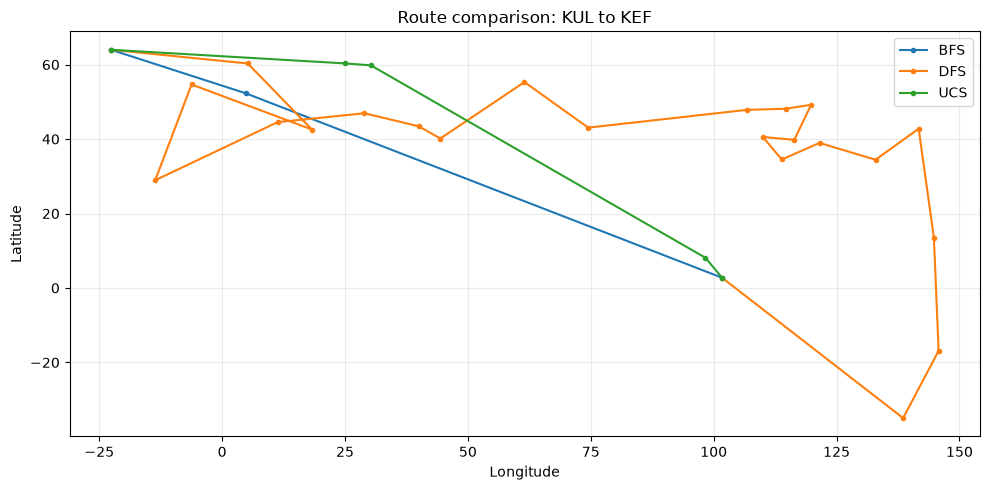
\includegraphics[width=.88\linewidth,height=5cm,keepaspectratio]{labs/visuals/01-notebook-reference.png}
\end{labvisual}
\begin{refoutput}
\begin{lstlisting}[style=utpterminal]
Saved: ['metrics.csv', 'route_comparison.png']
\end{lstlisting}
\end{refoutput}

\textbf{Read the result.} Regenerate this plot rather than copying it. Check the axes and the three routes; this saved figure is a reference, not evidence of your own run.
\end{labanswer}

\begin{yourturn}
Add new cells at the end of the notebook for these three tasks, and record your numbers before reading the expected findings.
\begin{enumerate}
  \item \textbf{Try a new query.} Run all three algorithms from \texttt{JFK} to \texttt{SYD} and record hops, kilometres and expansions.
  \item \textbf{Does direction matter?} Run BFS and UCS from \texttt{KEF} back to \texttt{KUL} and compare with the outward results. Is the best route back the same route reversed?
  \item \textbf{Check your warm-up.} Type in the graph of \figref{fig:ucs-vs-bfs} and compare with your hand trace. Then remove the edge from D to G and predict what BFS returns.
\end{enumerate}
\begin{lstlisting}[style=utppython]
tiny = {"A": [("B", 1.0), ("C", 4.0)], "B": [("D", 3.0), ("E", 2.0)], "C": [("F", 5.0)],
        "D": [("G", 4.0)], "E": [("G", 1.0)], "F": [("G", 2.0)], "G": []}
print(bfs(tiny, "A", "G").path, ucs(tiny, "A", "G").path)
\end{lstlisting}
\end{yourturn}

\begin{expectedfindings}
\begin{enumerate}
  \item BFS: 2 hops, 23,093~km via AUH, 537 expanded. DFS: 45 hops, 64,251~km. UCS: 2 hops, 16,035~km via LAX, 3,097 expanded. BFS stops at the first two-leg route it meets, 7,000~km too long.
  \item BFS: 2 hops via AMS, 12,274~km. UCS: 4 hops via HEL, LED and TAS, 11,478~km, which is not the outward UCS route reversed. Routes are directed, so a route out does not guarantee the same route back.
  \item BFS returns A--B--D--G at cost 8 and UCS returns A--B--E--G at cost 4. With the edge from D to G removed, BFS also returns A--B--E--G, because that is now the first three-edge route it reaches.
\end{enumerate}
\end{expectedfindings}

\begin{troubleshoot}
\begin{description}
  \item[\texttt{ModuleNotFoundError: utils}] Jupyter was not started from \texttt{all\_experiments/}. Restart it from there, or run the script from the course folder.
  \item[\texttt{FileNotFoundError}] A data file is missing or misnamed. Match Chapter~\ref{ch:toolkit}'s names, capitals too.
  \item[Different counts from the reference] Use the supplied data files and an unedited \texttt{utils/core.py}. Runtimes vary by machine; hops, kilometres and expansions should not.
\end{description}
\end{troubleshoot}

\begin{verification}
\begin{itemize}
  \item The cleaned graph has 6,464 usable airports and 37,337 unique directed routes.
  \item Every BFS, DFS and UCS path uses real routes, and its cost is the sum of its legs.
  \item BFS returns the fewest hops and UCS the shortest distance on every query; UCS finds the 11,461~km KUL$\to$KEF route.
  \item Reversing the neighbour order changes the DFS route, and you can explain why.
  \item \texttt{results/lab01/} holds \texttt{metrics.csv} and \texttt{route\_comparison.png}.
\end{itemize}
\end{verification}

\begin{labdeliverable}
\begin{itemize}
  \item Restart the kernel and run all cells without errors.
  \item Submit the executed notebook, including your \emph{Your turn} cells, and the generated \texttt{results/lab01/} folder.
  \item Add a short conclusion: which method minimises hops, which minimises distance, why DFS changes with neighbour order, and which effort measure is comparable across computers.
\end{itemize}
\end{labdeliverable}

